\section{Présentation du projet}

\subsection{Origine et nature du projet }
\setlength{\parindent}{5ex}
Étant tous passionnés des jeux vidéo, il était évident que nous voulions créer un jeu vidéo pour ce projet. Notre idée n'était pas de privilégier les graphismes de notre jeu étant donné qu'il s'agissait de notre premier projet et qu'on ne voulait pas centrer nos efforts dans la partie graphique mais plutôt dans la partie jouable. Après avoir considéré le genre "bullet hell", on a finalement opté de créer un jeu d'horreur psychologique: \textbf{Nyctalopia}.

\subsection{Objet de l’étude}
\setlength{\parindent}{5ex}
Nous pensons que ce projet peut nous aider dans bien des domaines qui nous serons utiles dans notre vie professionnelle, c'est notre premier projet de groupe dans lequel on va devoir assumer des responsabilités, faire face à des problèmes et rendre un produit de bonne qualité, le tout en respectant des critères donnés.
\newline\indent
En effet, ce projet nous apportera une première expérience d'un travail en groupe sur une grande période et nécessitant une rigueur de travail conséquente, pratique courante d'un ingénieur.
\newline\indent
Ce projet nous permettra de mettre en pratique ce que nous avons appris en Travaux Pratiques et demandera un travail de recherche important demandant de l'autonomie et de l'indépendance.


\subsection{État de l’art}
\setlength{\parindent}{5ex}
Le premier jeu d'horreur nommé \emph{Haunted House} sort en 1972 avec la première console de salon, la Magnavox Odyssey. Il s'agit d'un jeu de poursuite à deux joueurs joué sur une maison hantée, il est sorti en 1972. Le détective tâtonne dans l'obscurité, rassemblant tous les indices possibles, alors qu'il se dirige vers le trésor au dernier étage de la maison hantée le tout en évitant l'autre joueur. Cette méchanique chasseur/chassé sera reprise plus tard dans les premiers jeux d'horreurs 3D et continue de nos jours à être très utilisée dans le genre.

Notre inspiration provient de jeux comme \emph{Silent Hill}, \emph{Resident Evil} ou \emph{Phasmophobia} des jeux qui sont devenus aujourd'hui une référence dans le monde des jeux d'horreur et on établit des règles propres à ce genre.

\emph{Silent Hill} avec son environnement effrayant arrivait déjà en 1999 à produire une sensation d'angoisse et de frisson dans une époque dans laquelle la capacité graphique était très limitée par les avancées technologiques (\emph{fig. 1}).

\vfill
\noindent\makebox[\linewidth]{\rule{.8\paperwidth}{.6pt}}\\[0.2cm]
EPITA Toulouse - Projet S2 - 2021/2022 \hfill Nyctalopia - gameHUB
\noindent\makebox[\linewidth]{\rule{.8\paperwidth}{.6pt}}

\begin{figure}[H]
\centering
\begin{minipage}{.5\textwidth}
  \centering
  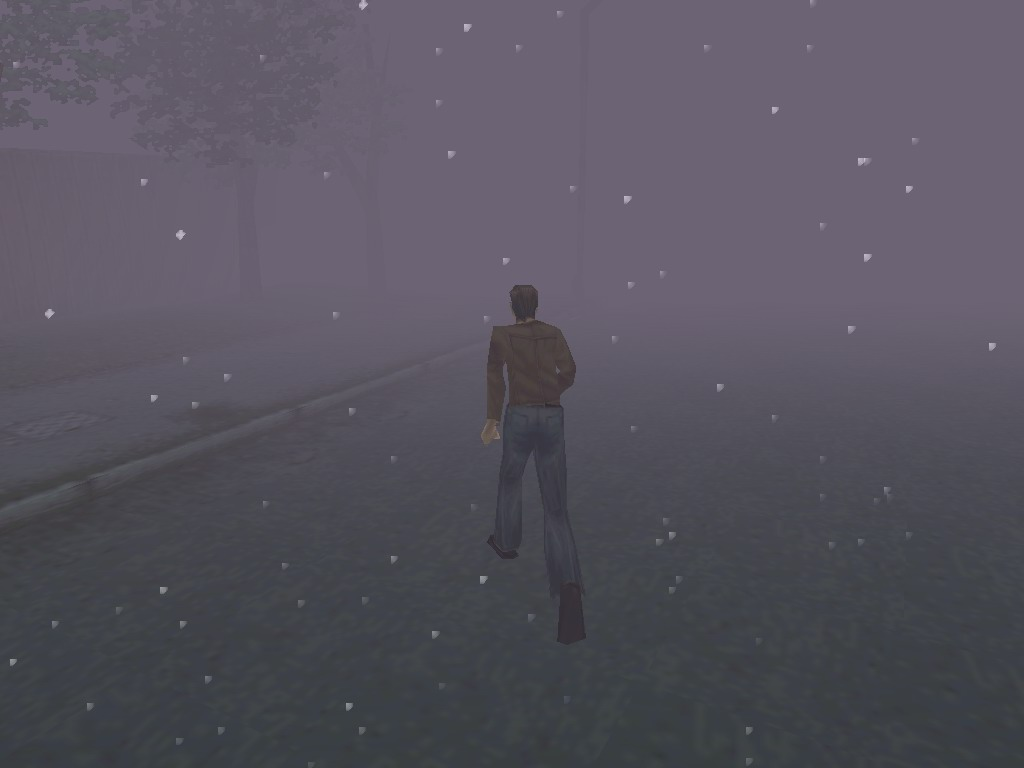
\includegraphics[width=.6\linewidth]{img/silenthill.jpg}
  \captionof{figure}{\emph{Silent Hill, Konami 1999}}
  \label{fig:silenthill}
\end{minipage}%
\begin{minipage}{.5\textwidth}
  \centering
  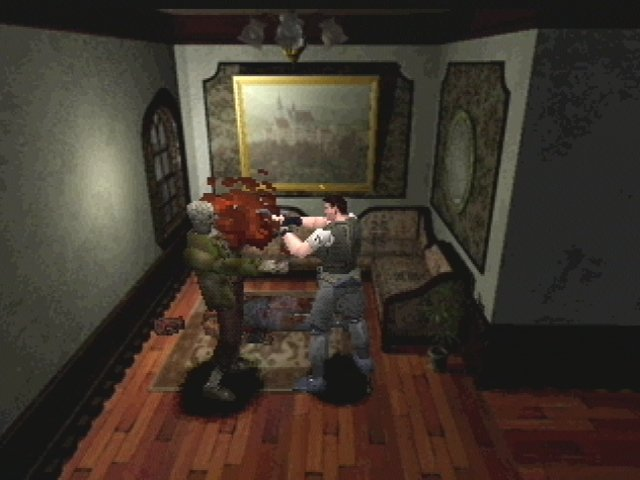
\includegraphics[width=.6\linewidth]{img/residentevil.jpg}
  \captionof{figure}{\emph{Resident Evil, Capcom 1996}}
  \label{fig:residentevil}
\end{minipage}
\end{figure}

\emph{Resident Evil} développé par Shinji Mikami et Tokuro Fujiwara pour \emph{Playstation 1} (\emph{fig. 2}), est un des plus connus jeux du type \emph{survival horror} qui mélange l'action avec la thématique d'horreur, le but étant de mettre en place une mécanique de gestion de ressources que le joueur doit tenir en compte pour survivre. 

\emph{Phasmophobia}, un jeu indépendant développé par \emph{Kinetic Games} sur Unity utilise de manière très pertinente et révolutionnaire un chat vocal par proximité. Dans ce jeu coopératif, les joueurs ne peuvent s'entendre que s'ils se trouvent près les uns des autres. Ce chat vocal permet non seulement d'interagir avec les différentes entités qui nous suivent dans le jeu mais aussi de créer des situations dans lesquelles les joueurs, devant se séparer, se retrouvent seuls dans un environnement menaçant.

Tous ces jeux ont un point commun, ils ont tous une caractéristique particulière qui leur rendent effrayants: le fait d'avoir peur par l'ambiance dans laquelle le joueur est placé, la peur de n'avoir plus de munitions dans son arme ou la peur de rester seul sachant que il y a un ennemi qui nous hante.

Nyctalopia cherche à être un jeu qui laisse voler l'imagination du joueur, l'objectif principal n'étant pas de faire courir un monstre derrière les joueurs. On cherchera à travers les effets, le son et les environnements, de créer une ambiance lugubre qui, comme sur les jeux précédemment cités, rendent le joueur mal à l'aise. 

\vfill
\noindent\makebox[\linewidth]{\rule{.8\paperwidth}{.6pt}}\\[0.2cm]
EPITA Toulouse - Projet S2 - 2021/2022 \hfill Nyctalopia - gameHUB
\noindent\makebox[\linewidth]{\rule{.8\paperwidth}{.6pt}}

\subsection{Moyens technologiques requis}
Les moyens technologiques requis correspondent notamment aux logiciels
nécessaires pour le développement du projet. Le principal est le moteur de jeu Unity3D comme base du jeu, puis vient Blender3D pour la création et/ou modification de modèles 3D. 

Un logiciel de traitement d’image sera également nécessaire, pour créer les images qui seront utilisées comme le logo ou les textures. Un logiciel tel que Adobe Photoshop ou GIMP devra être utilisé. 

L’environnement de développement JetBrains Rider sera quant à lui utilisé pour le développement des scripts en C\# qui feront fonctionner le jeu. Pour développer le mode multijoueur,la bilbliothèque Unity Multiplayer Services Beta sera envisagée afin de simplifier le processus d'intégration.


Pour réaliser le cahier des charges ou les différents rapports de soutenances, l'éditeur \LaTeX  en ligne Overleaf sera employé.


Enfin, pour travailler en groupe, le logiciel de contrôle de version GitHub sera utilisé, permettant de suivre à la trace chaque évolution du projet avec les modification de chaque étudiants du groupe.

\subsection{Les coûts}
En tant qu'étudiants, nous sommes réputés pour être "sans-le-sou", ce qui complique grandement la tâche de réaliser des projets. Heureusement pour nous, les logiciels ou assets utilisés sont tous créés par nos soins, gratuits, Open Source, ou bien avec licence spéciale étudiante fournie par EPITA, ce qui limite grandement les coûts.
Le nom de domaine, est offert grâce au GitHub Student Pack pendant 1 an, suffisant pour le projet.

\vfill
\noindent\makebox[\linewidth]{\rule{.8\paperwidth}{.6pt}}\\[0.2cm]
EPITA Toulouse - Projet S2 - 2021/2022 \hfill Nyctalopia - gameHUB
\noindent\makebox[\linewidth]{\rule{.8\paperwidth}{.6pt}}

\newpage